A promising approach for improving reliability of software is \emph{formal verification}, in which
a system is developed along with a proof that it always follows a high-level
specification of its intended behavior. The first contribution of this
thesis is to develop ideas and techniques for formal verification of a class of
systems that store persistent data. The key challenges in such systems are that
they make guarantees about \emph{crashes} where the whole computer stops and
reboots, and that their implementations take advantage of \emph{concurrency} for
good performance.

The thesis applies these verification techniques to a \emph{file system},
the service in an operating system that implements the abstraction of files and
directories. File systems are important because they are used by all
applications to store data, and bugs in file systems are especially costly
because they can lead to data loss for any of these applications. This thesis
also contributes a design and approach that isolate crash and concurrency
reasoning to a transaction system, so that the majority of the file system is
verified with much simpler sequential reasoning.

\section{Motivation}
\label{sec:intro:motivation}

Systems that store persistent data are challenging to make correct; concurrency
on its own is hard to reason about, and the possibility of a crash at any time
makes it more difficult. File systems are a good instance of such a system where
handling concurrency and crashes is important for correctness.

A file system is an especially critical system for
three reasons. First, the file system is widely used --- essentially all applications have
data that is ultimately stored in a file system. Second, implementations are
concurrent and optimized to improve performance, which increases the potential
for bugs. Finally, bugs are particularly costly since they can lead to permanent
data loss for any application running on top.

Crashes and
concurrency are the key challenges in writing a correct file system.
A file system is generally expected to keep application data safe
even if the system stops running at any time, say due to a power failure or
kernel panic. This thesis uses ``crash'' to refer to any of these circumstances
where the computer stops and is rebooted. After a reboot, the file system is
expected to preserve data from before the crash. The second big challenge is
concurrency in the implementation. Both challenges complicate testing, fuzzing,
and verification. The combination of concurrency and crashes can also lead to more
intricate and hard-to-find bugs.

Even in widely used file systems like ext4 and btrfs, new bugs are still discovered,
despite a long history of developing, testing, and using these file systems. For
example, a
recent approach for fuzzing file systems~\cite{kim:hydra} found new crash-safety
issues in both ext4 and btrfs, despite not testing for concurrency issues. A
study conducted in 2013 looked at all patches for Linux file systems from
2005--2013~\cite{lu:fsstudy}, finding hundreds of these patches were to fix bugs
(for example, 450 for ext4 and 358 for btrfs). About 60\% of these bugs lead to
data loss or crash the kernel (and as the study points out, these are much more
serious consequences than most bugs in application software). File systems have
a lot of internal concurrency for performance reasons, which both leads to bugs
and makes testing and fuzzing more challenging.

This thesis develops techniques to apply formal verification to a file system,
which has the potential to completely eliminate whole classes of bugs.
In this approach, we write the code, then a specification of the
intended behavior of the code, and finally a mathematical proof that shows the
code always meets the specification. For confidence in the proof itself, the
proof is carried out with a computer and a piece of software called a proof
assistant checks that the proof is valid. The nature of formal verification
forces the proof engineer to systematically cover every corner case in the code.
As a result, verification can rule out whole classes of bugs, including
low-level bugs like memory safety but also logic errors like returning the wrong
data. Verification does not guarantee that a system is bug-free, because the
specification must be correct and the assumptions in the proof must hold in
practice, but it does help since the specification is intended to be easier to
understand than the implementation, and verification isolates debugging to
identifying where the specification is wrong or an assumption was violated.

% The key to verifying a system with the complexity of DaisyNFS is a design
% that splits the file system into two main parts: a transaction system called
% GoTxn that makes it easy to get atomicity over the disk, and then the rest of
% the file system implemented using a transaction per operation. GoTxn must face
% the key challenges of crash safety and concurrency, but it handles them in such
% a way that the code on top is verified using comparatively much simpler
% sequential reasoning. The file-system code then focuses on implementing features
% like the details of the NFS semantics, large files, and efficient data
% structures.

\section{State of the art}
\label{sec:intro:related}

While the idea of formal verification is not new, there was essentially no
support for reasoning about the combination of crashes and concurrency when this
thesis work started (in 2015). Thus this thesis develops new techniques to
reason about the combination in the first place. We apply these techniques to
DaisyNFS, a verified implementation of the Network File System (NFS) protocol, a
standard file-system interface.

Production file systems are generally validated by testing. While testing is
indispensable for development, the nature of a file system makes it difficult to
catch all bugs with only testing. The fundamental difficulty is a high degree of
non-determinism from two sources: crashes in the middle of execution, and
concurrency in the implementation that is needed for good performance. This
leads to many possible execution paths, which are difficult to exhaustively test.

The importance of file-system correctness has been recognized by the academic
community, thus there are many approaches for increasing confidence with
improved testing. One line of work has explored systematically testing crashes
at intermediate points~\cite{mohan:crashmonkey,pillai:appcrash,yang:explode}. Another line of
work has focused on fuzz testing as a way to induce crash-safety
bugs~\cite{xu:janus,kim:hydra}. These approaches have been successful for
finding bugs, including crash-safety bugs, but they only test sequential
executions, missing bugs due to concurrently issued operations or from crashes
that interrupt multiple operations. Furthermore, unlike formal verification, testing cannot
cover all executions of a program, even without crashes and concurrency,
potentially missing bugs.

The research community has also recognized the value of formal verification for
reasoning about a file-system implementation. The closest related work
(carried out concurrently with the work in this thesis) is
Flashix~\cite{bodenmuller:concurrent-flashix}, a verified, concurrent file
system that runs on flash devices. The methodology used in the proof is
different from the Perennial logic we developed, as is the Flashix artifact from
the DaisyNFS file system described in this thesis. See \cref{sec:rel:flashix}
for a more detailed explanation.

There are other verified file systems, especially the sequential file systems
FSCQ~\cite{chen:fscq} and Yggdrasil~\cite{sigurbjarnarson:yggdrasil} and an
concurrent but in-memory file system AtomFS~\cite{zou:atomfs}. These systems use
verification techniques that do not support both crashes and concurrency, and they
cannot be extended them in a straightforward way to support the other form of reasoning.

\section{Approach}
\label{sec:intro:approach}

What does it mean to give a machine checked, formal proof of a system? At a high
level, program proofs always have three components: an implementation, a
specification, and a proof. When doing machine-checked proofs, all three are
physically represented as code in a verification system. The verification system
checks the proof against the implementation and specification, ensuring that the
proof is complete.
This thesis integrates interactive, foundational proofs using custom
infrastructure (in Coq~\cite{coq}) as well as automated verification using a
verification-aware programming language (Dafny~\cite{leino:dafny}). These are
both machine-checked, formal proofs, but the interaction models of the two
systems are different enough that this section describes them separately.
\Cref{fig:overview} gives a high-level overview of how the pieces fit together,
which this section introduces bit by bit. The system and proof are divided into
two parts: the lower half of the figure represents GoTxn, a verified transaction
system implemented in the Go programming language~\cite{lang:go} (in the lower
left of the figure) and verified in Coq (in the lower right), while the upper
half represents the remaining file-system code implemented and verified in
Dafny.

\begin{figure}[ht]
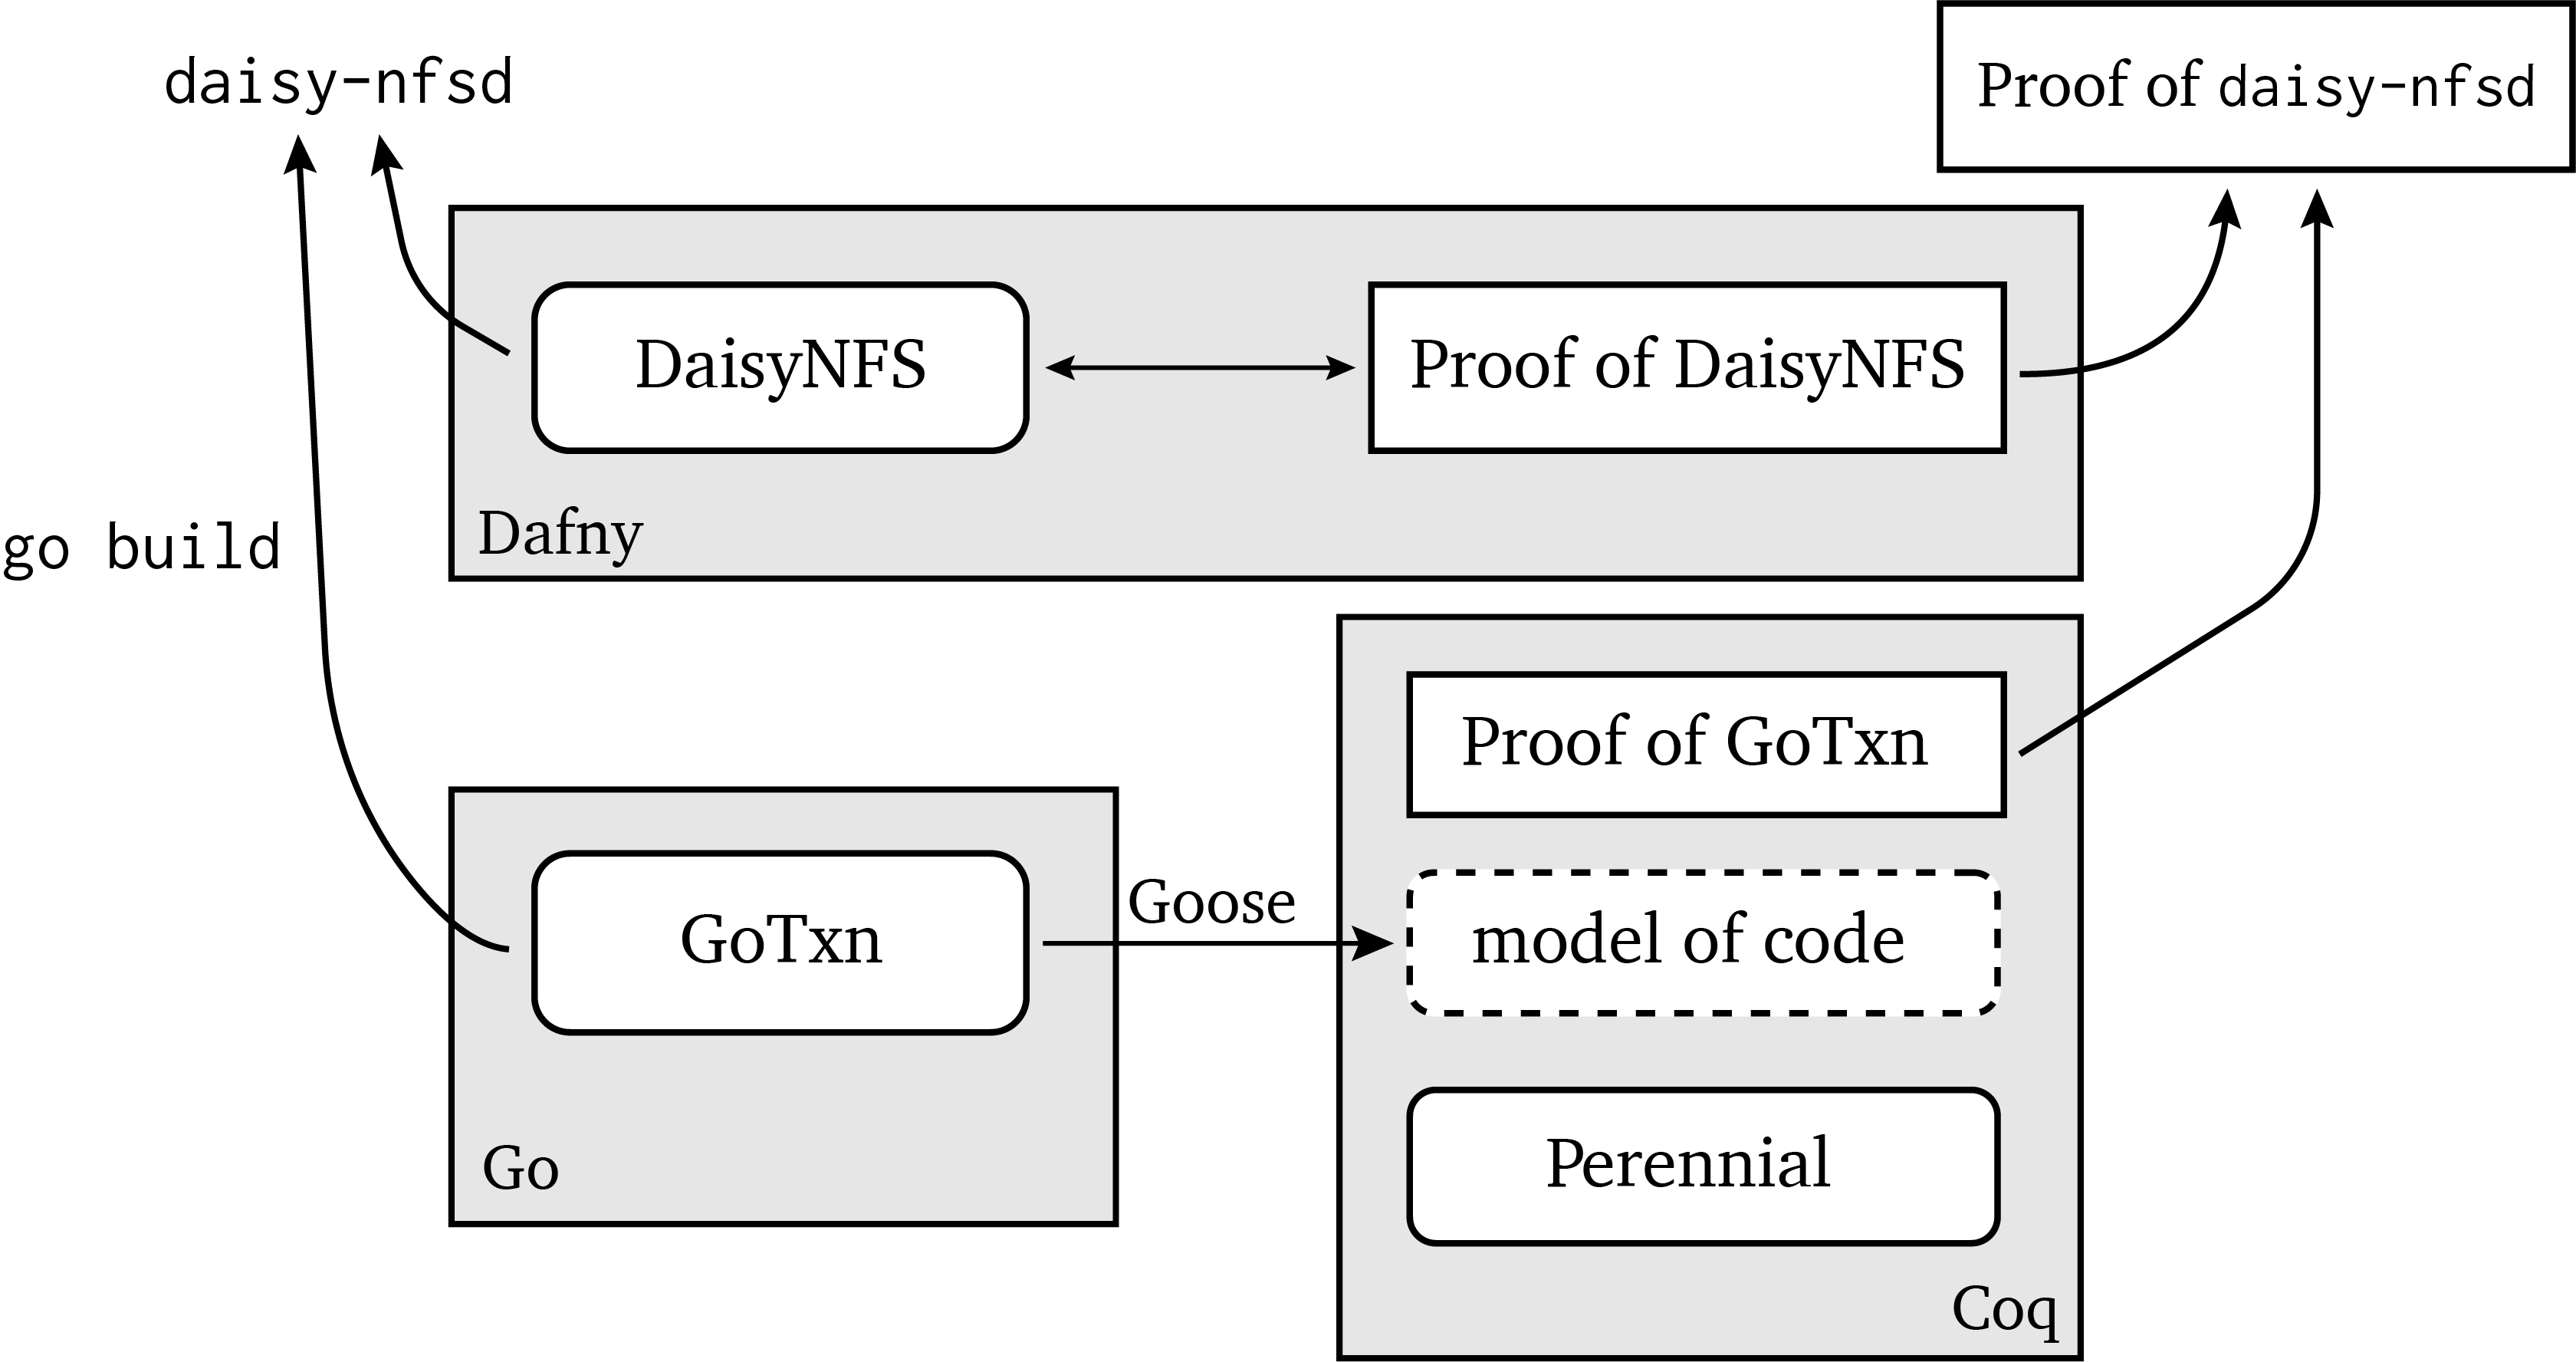
\includegraphics{fig/overview.png}
\caption{Overview of how GoTxn, DaisyNFS, and the proofs fit together.}
\label{fig:overview}
\end{figure}

\paragraph{Goose to model GoTxn in Coq.}
In Coq, the core feature is proofs based on dependent type theory, which is
expressive enough to represent essentially any math. The first step when using
Coq is to connect the Go code implementing the GoTxn library to the reasoning in
the proof assistant. The particular approach in this thesis translates
executable code to a model in Coq, implemented by a new tool called Goose. The model
encodes the assumptions the proof makes about how the program behaves in the
form of a semantics, structured as a transition system. For GoTxn, this
transition system describes its execution as a sequence of states the program
might go through along with return values from the library's methods.

\paragraph{The Perennial program logic.}
Once we have GoTxn modeled in Coq, we can reason about it. The goal of
verification is to prove that all possible behaviors of the program are allowed
by its specification. The specifications in this work forbid universally
incorrect behavior, like reading an out-of-bounds address in an array, but also
precisely specifies what the program is supposed to do. GoTxn has a particularly
interesting specification that describes how it makes transactions appear to
execute atomically, described in greater detail in \cref{ch:txn}.

GoTxn has a large implementation, so it would be challenging to a direct proof
reasoning about all of its behaviors.
A common structure to tame the complexity of reasoning about a program is to use
a \emph{program logic}. In principle it might be possible to do this reasoning
directly, but in practice such a proof would too
complex to be feasible. The program logic organizes the proof with a structured
way of expressing and proving statements about the program, such as breaking the
proof down into theorems about individual functions. The proof in a program
logic will often mirror the structure of the code, since each function has its
own specification and groups of related functions have related specs.

Program logics for concurrency are still an active area of research; only
recently have they reached the maturity to give completely mechanized proofs of
moderate-sized programs. There are few logics that also can reason about crash
safety. Our approach in this thesis is to build a new program logic called Perennial with all the
concurrency-reasoning features of a modern program logic, plus new features for
reasoning about crashes. In \cref{fig:overview}, Perennial appears in the bottom
of the Coq shaded box, since it is the basis for the GoTxn proofs. Perennial builds upon Iris, a modular framework for
concurrency, preserving its concurrency features while extending it with
crash-safety reasoning.

\paragraph{Verifying GoTxn.}
Using the new Perennial program logic, we verified GoTxn, a concurrent
transaction system.
The transaction system's correctness theorem says that any program that uses
transactions really has transactional behavior: its execution is equivalent to a
version of the program where the transactions run atomically. The complete
specification includes some important details in order to formalize the
intuition behind atomicity. GoTxn is a general-purpose library for transactions,
and could be used independently for another storage system.

Because every transaction appears to run sequentially and persist its writes to
disk all at once, it is no longer necessary to use a sophisticated program logic
like Perennial to reason about the body of each transaction. Instead, we switch
to using Dafny, a verification-oriented programming language that only supports
sequential code but as a result is highly productive for this use case. The file
system is written and verified in Dafny, then compiled to Go and linked with
GoTxn.

\paragraph{Implementing and verifying DaisyNFS in Dafny.}
The top half of \cref{fig:overview} depicts the implementation and proof for the
DaisyNFS file-system code, implemented on top of GoTxn in the Dafny programming language.
Dafny verification works quite differently from Coq. Dafny is a programming
language with verification features; contrast this with Coq, which supports
general math that can \emph{model} programs. A Dafny method can be annotated
with a specification. The Dafny checker converts a method and its specification
to a logical formula (called a verification condition), which is true if and only if the specification holds for
the method. It then queries a \emph{solver} (Z3, in the case of Dafny) to determine if the formula is true.
Contrast all of this with Coq, where the user manually develops the program
logic and connects the rules of this logic. Checking a program against its specification in Dafny cannot be perfectly
automated because it is impossible to answer whether a general logical formula
is true or not, but the user can insert annotations to help out the solver, and
generally fewer annotations are needed than lines of proof for Coq. The main
downside to this approach is that it fixes a sequential programming language, so
unlike in Coq, it isn't possible to reason about concurrency and crashes.

\paragraph{Linking the code and proofs together.}
Outside of the Go, Coq, and Dafny boxes in \cref{fig:overview} are two outputs,
one for the implementation and another for the proof.
The left-hand side depicts the implementation, split between GoTxn
and the file-system implemented in Dafny. The Dafny code is compiled to Go and
then the two parts are linked together into one \cc{daisy-nfsd} binary in the
usual Go build process.

The right-hand side of the figure depicts all aspects related to the
proof. The GoTxn proof is carried out in the Coq proof assistant, which checks
that the proofs are valid.
Meanwhile
the DaisyNFS file-system code is verified in Dafny, which integrates
implementing, specifying, and verifying code. This proof is checked by the Dafny
verifier. Finally, the proof of GoTxn is written in such a way that it can be
composed with the proof of DaisyNFS for a theorem about the whole
\cc{daisy-nfsd} binary. This is a conceptual composition, not one in either
Dafny or Coq, which is described in greater detail in \cref{ch:daisy-nfs}.

One of the contributions of this thesis is that the file-system design isolates
concurrency and crash safety into the transaction system. The rest of the system
implements the file-system logic and data structures. Because each operation is
wrapped in a transaction that appears to run sequentially and without crashes,
we use Dafny for this implementation and proof. Intuitively what the file-system
proof shows is that it correctly implements the NFS protocol: the
\cc{daisy-nfsd} server binary appears to atomically respond to requests
according to (a mathematical description of) the NFS protocol, despite
concurrent requests and even if the system crashes.

In order to connect the file system's sequential proofs to its concurrent
execution, we prove a general theorem about the transaction system's
implementation. The starting point is the idea of a \emph{simulation} proof,
which shows that a system like the file-system transactions correctly implement an
abstract specification like the NFS protocol. The GoTxn
\emph{simulation-transfer theorem} shows that for any system implemented using
transactions with a sequential simulation proof, the concurrent system running
with GoTxn concurrently simulates its abstract specification where each
operation is atomic. Intuitively this theorem holds because every concurrent
execution of the GoTxn transactions appears to be atomic, and then the
sequential simulation proof shows those atomic transactions implement the
abstract specification. However, the GoTxn theorem formalizes precisely what
conditions are required for the simulation transfer, including restrictions on
the transactions and exactly what crash safety guarantees are achieved. Note
that the simulation-transfer theorem is a general property of GoTxn that this
thesis applies to DaisyNFS but which could also be applied to other verified
storage systems.

\section{Contributions}
\label{sec:intro:contributions}

This thesis makes the following contributions:

\paragraph{New verification foundations.}
\textbf{Perennial} is a program logic for crash safety
and concurrency using specifications based on crash weakest
preconditions. These include crash conditions combined with concurrency
and reasoning principles for moving ownership to a recovery procedure
following a crash. \textbf{Logically atomic crash specifications} are a
pattern using Perennial's crash weakest preconditions for specifying
libraries that have both concurrent behavior and involve persistent
state. These are implemented using Perennial and used in the GoTxn
proof.

\paragraph{Reasoning about storage systems.}
GoTxn has a new \textbf{lifting-based specification} for its journaling
layer to reason about concurrent transactions separately, which is
challenging since the logical disk can change in the middle of a transaction. Its proof uses a novel
\textbf{history-based abstract state} for the write-ahead log. This model allowed us to carry
out a modular proof where the write-ahead logging library hides most of
its internal complexity, simplifying reasoning about the rest of the GoTxn
code that uses it. Finally, GoTxn exports a \textbf{transaction refinement}
specification that captures how transactions appear to run atomically.

\paragraph{Verifying efficient code.}
\textbf{Goose} connects efficient code implemented in Go to a model of that code
in Perennial. A general contribution here is a design for systems verification
that enables efficient code and convenient reasoning. Goose includes reasoning
principles for the models that it outputs, to support verifying the translated
code.

\paragraph{System design.}
DaisyNFS is verified using sequential code despite having a concurrent
implementation. The formal justification for this approach is a
\textbf{simulation-transfer theorem}, proven on top of GoTxn's
transaction-refinement specification, which shows that sequential reasoning for each
transaction in a system implies correctness for the whole system when run on top
of GoTxn. Sequential reasoning means DaisyNFS can be verified using Dafny, a
sequential verification language, with much lower proof burden than would
otherwise be possible. The specification for DaisyNFS uses a mathematical
formulation of RFC 1813, the document that (in prose) specifies what a NFSv3
server should do.

The ideas in Perennial and Goose are applied to GoTxn, but they could be used
for reasoning about other concurrent storage systems. Similarly,
this thesis uses GoTxn to build a verified file system, but it could also be used
as the basis for other verified storage systems, like a persistent key-value
store.

The techniques and artifacts in this thesis do have some limitations, described
in more detail in the appropriate chapters. Some examples include: Perennial can reason
about safety but not liveness (see \cref{sec:perennial:limitations}); GoTxn does
not support asynchronous durability (see \cref{sec:txn:limitations}); DaisyNFS
lacks support for symbolic links (see \cref{sec:daisy:motivation}); and Goose
does not support Go's channels or interfaces (see \cref{sec:goose:limitations}).

\section{Reading guide for the thesis}
\label{sec:intro:reading-guide}

This section briefly outlines the chapters of the thesis, the dependencies
between chapters, and the intended audience. Broadly the thesis is intended for
a systems audience, except for the verification foundations. The support for
concurrency makes all of the formal underpinnings in the thesis more technical
than foundations for sequential systems verification.

\Cref{ch:related} covers related work across Perennial, GoTxn, and DaisyNFS, for
a broad computer-science audience. To keep the Goose chapter self-contained, its
related work is described in the relevant chapter.

\Cref{ch:perennial} is an overview of Perennial. This chapter is oriented
towards a reader interested in the verification underpinnings and not
necessarily the systems side. At this level of abstraction Perennial is
independent of both the GoTxn proof and even Goose for verifying Go code. Some
experience with program logics is helpful for understanding the presentation.

\Cref{ch:crash-logatom} describes a style of logically atomic specifications
that capture both concurrency and crash atomicity using Perennial. It uses an
extended example from the GoTxn proof and explains its formal underpinnings at a
high level. This is the most technically involved chapter.

\Cref{ch:txn} describes the design and proof of GoTxn. An important part of GoTxn is its
specification, which captures how transactions are atomic. This chapter does not
require the full Perennial or logical atomicity chapters.

\Cref{ch:daisy-nfs} describes the design and proof of DaisyNFS.\@ This chapter
explains the proof approach that justifies using Dafny to verify DaisyNFS even
though Dafny is a sequential verification tool and DaisyNFS is a concurrent
system.

\Cref{ch:goose} is about Goose and talks about verifying Go code generally, with
nothing specific to GoTxn or even storage systems. This is the first detailed
description of Goose, so this chapter is written to be readable without any of
the other chapters.

\Cref{ch:impl} is a short chapter covering some implementation details in
DaisyNFS, covering both GoTxn and the file-system code.

\Cref{ch:eval} evaluates the whole file system along a few dimensions,
especially performance but also aspects of the proof.

\Cref{ch:conclusion} concludes with some discussion about the broader value of
verification, lessons learned, and future work.
